\documentclass[1p]{elsarticle_modified}
%\bibliographystyle{elsarticle-num}

%\usepackage[colorlinks]{hyperref}
%\usepackage{abbrmath_seonhwa} %\Abb, \Ascr, \Acal ,\Abf, \Afrak
\usepackage{amsfonts}
\usepackage{amssymb}
\usepackage{amsmath}
\usepackage{amsthm}
\usepackage{scalefnt}
\usepackage{amsbsy}
\usepackage{kotex}
\usepackage{caption}
\usepackage{subfig}
\usepackage{color}
\usepackage{graphicx}
\usepackage{xcolor} %% white, black, red, green, blue, cyan, magenta, yellow
\usepackage{float}
\usepackage{setspace}
\usepackage{hyperref}

\usepackage{tikz}
\usetikzlibrary{arrows}

\usepackage{multirow}
\usepackage{array} % fixed length table
\usepackage{hhline}

%%%%%%%%%%%%%%%%%%%%%
\makeatletter
\renewcommand*\env@matrix[1][\arraystretch]{%
	\edef\arraystretch{#1}%
	\hskip -\arraycolsep
	\let\@ifnextchar\new@ifnextchar
	\array{*\c@MaxMatrixCols c}}
\makeatother %https://tex.stackexchange.com/questions/14071/how-can-i-increase-the-line-spacing-in-a-matrix
%%%%%%%%%%%%%%%

\usepackage[normalem]{ulem}

\newcommand{\msout}[1]{\ifmmode\text{\sout{\ensuremath{#1}}}\else\sout{#1}\fi}
%SOURCE: \msout is \stkout macro in https://tex.stackexchange.com/questions/20609/strikeout-in-math-mode

\newcommand{\cancel}[1]{
	\ifmmode
	{\color{red}\msout{#1}}
	\else
	{\color{red}\sout{#1}}
	\fi
}

\newcommand{\add}[1]{
	{\color{blue}\uwave{#1}}
}

\newcommand{\replace}[2]{
	\ifmmode
	{\color{red}\msout{#1}}{\color{blue}\uwave{#2}}
	\else
	{\color{red}\sout{#1}}{\color{blue}\uwave{#2}}
	\fi
}

\newcommand{\Sol}{\mathcal{S}} %segment
\newcommand{\D}{D} %diagram
\newcommand{\A}{\mathcal{A}} %arc


%%%%%%%%%%%%%%%%%%%%%%%%%%%%%5 test

\def\sl{\operatorname{\textup{SL}}(2,\Cbb)}
\def\psl{\operatorname{\textup{PSL}}(2,\Cbb)}
\def\quan{\mkern 1mu \triangleright \mkern 1mu}

\theoremstyle{definition}
\newtheorem{thm}{Theorem}[section]
\newtheorem{prop}[thm]{Proposition}
\newtheorem{lem}[thm]{Lemma}
\newtheorem{ques}[thm]{Question}
\newtheorem{cor}[thm]{Corollary}
\newtheorem{defn}[thm]{Definition}
\newtheorem{exam}[thm]{Example}
\newtheorem{rmk}[thm]{Remark}
\newtheorem{alg}[thm]{Algorithm}

\newcommand{\I}{\sqrt{-1}}
\begin{document}

%\begin{frontmatter}
%
%\title{Boundary parabolic representations of knots up to 8 crossings}
%
%%% Group authors per affiliation:
%\author{Yunhi Cho} 
%\address{Department of Mathematics, University of Seoul, Seoul, Korea}
%\ead{yhcho@uos.ac.kr}
%
%
%\author{Seonhwa Kim} %\fnref{s_kim}}
%\address{Center for Geometry and Physics, Institute for Basic Science, Pohang, 37673, Korea}
%\ead{ryeona17@ibs.re.kr}
%
%\author{Hyuk Kim}
%\address{Department of Mathematical Sciences, Seoul National University, Seoul 08826, Korea}
%\ead{hyukkim@snu.ac.kr}
%
%\author{Seokbeom Yoon}
%\address{Department of Mathematical Sciences, Seoul National University, Seoul, 08826,  Korea}
%\ead{sbyoon15@snu.ac.kr}
%
%\begin{abstract}
%We find all boundary parabolic representation of knots up to 8 crossings.
%
%\end{abstract}
%\begin{keyword}
%    \MSC[2010] 57M25 
%\end{keyword}
%
%\end{frontmatter}

%\linenumbers
%\tableofcontents
%
\newcommand\colored[1]{\textcolor{white}{\rule[-0.35ex]{0.8em}{1.4ex}}\kern-0.8em\color{red} #1}%
%\newcommand\colored[1]{\textcolor{white}{ #1}\kern-2.17ex	\textcolor{white}{ #1}\kern-1.81ex	\textcolor{white}{ #1}\kern-2.15ex\color{red}#1	}

{\Large $\underline{12a_{0597}~(K12a_{0597})}$}

\setlength{\tabcolsep}{10pt}
\renewcommand{\arraystretch}{1.6}
\vspace{1cm}\begin{tabular}{m{100pt}>{\centering\arraybackslash}m{274pt}}
\multirow{5}{120pt}{
	\centering
	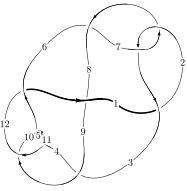
\includegraphics[width=112pt]{../../../GIT/diagram.site/Diagrams/png/1398_12a_0597.png}\\
\ \ \ A knot diagram\footnotemark}&
\allowdisplaybreaks
\textbf{Linearized knot diagam} \\
\cline{2-2}
 &
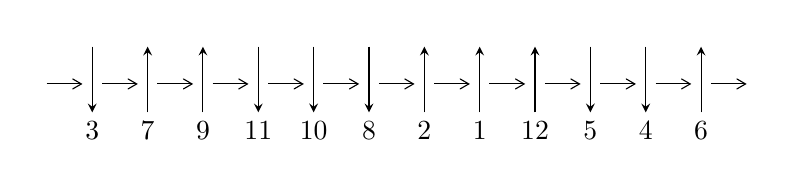
\begin{tikzpicture}[x=20pt, y=17pt]
	% nodes
	\node (C0) at (0, 0) {};
	\node (C1) at (1, 0) {};
	\node (C1U) at (1, +1) {};
	\node (C1D) at (1, -1) {3};

	\node (C2) at (2, 0) {};
	\node (C2U) at (2, +1) {};
	\node (C2D) at (2, -1) {7};

	\node (C3) at (3, 0) {};
	\node (C3U) at (3, +1) {};
	\node (C3D) at (3, -1) {9};

	\node (C4) at (4, 0) {};
	\node (C4U) at (4, +1) {};
	\node (C4D) at (4, -1) {11};

	\node (C5) at (5, 0) {};
	\node (C5U) at (5, +1) {};
	\node (C5D) at (5, -1) {10};

	\node (C6) at (6, 0) {};
	\node (C6U) at (6, +1) {};
	\node (C6D) at (6, -1) {8};

	\node (C7) at (7, 0) {};
	\node (C7U) at (7, +1) {};
	\node (C7D) at (7, -1) {2};

	\node (C8) at (8, 0) {};
	\node (C8U) at (8, +1) {};
	\node (C8D) at (8, -1) {1};

	\node (C9) at (9, 0) {};
	\node (C9U) at (9, +1) {};
	\node (C9D) at (9, -1) {12};

	\node (C10) at (10, 0) {};
	\node (C10U) at (10, +1) {};
	\node (C10D) at (10, -1) {5};

	\node (C11) at (11, 0) {};
	\node (C11U) at (11, +1) {};
	\node (C11D) at (11, -1) {4};

	\node (C12) at (12, 0) {};
	\node (C12U) at (12, +1) {};
	\node (C12D) at (12, -1) {6};
	\node (C13) at (13, 0) {};

	% arrows
	\draw[->,>={angle 60}]
	(C0) edge (C1) (C1) edge (C2) (C2) edge (C3) (C3) edge (C4) (C4) edge (C5) (C5) edge (C6) (C6) edge (C7) (C7) edge (C8) (C8) edge (C9) (C9) edge (C10) (C10) edge (C11) (C11) edge (C12) (C12) edge (C13) ;	\draw[->,>=stealth]
	(C1U) edge (C1D) (C2D) edge (C2U) (C3D) edge (C3U) (C4U) edge (C4D) (C5U) edge (C5D) (C6U) edge (C6D) (C7D) edge (C7U) (C8D) edge (C8U) (C9D) edge (C9U) (C10U) edge (C10D) (C11U) edge (C11D) (C12D) edge (C12U) ;
	\end{tikzpicture} \\
\hhline{~~} \\& 
\textbf{Solving Sequence} \\ \cline{2-2} 
 &
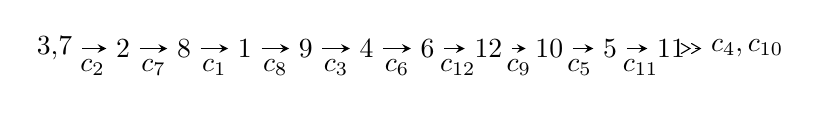
\begin{tikzpicture}[x=22pt, y=7pt]
	% node
	\node (A0) at (-1/8, 0) {3,7};
	\node (A1) at (1, 0) {2};
	\node (A2) at (2, 0) {8};
	\node (A3) at (3, 0) {1};
	\node (A4) at (4, 0) {9};
	\node (A5) at (5, 0) {4};
	\node (A6) at (6, 0) {6};
	\node (A7) at (7, 0) {12};
	\node (A8) at (8, 0) {10};
	\node (A9) at (9, 0) {5};
	\node (A10) at (10, 0) {11};
	\node (C1) at (1/2, -1) {$c_{2}$};
	\node (C2) at (3/2, -1) {$c_{7}$};
	\node (C3) at (5/2, -1) {$c_{1}$};
	\node (C4) at (7/2, -1) {$c_{8}$};
	\node (C5) at (9/2, -1) {$c_{3}$};
	\node (C6) at (11/2, -1) {$c_{6}$};
	\node (C7) at (13/2, -1) {$c_{12}$};
	\node (C8) at (15/2, -1) {$c_{9}$};
	\node (C9) at (17/2, -1) {$c_{5}$};
	\node (C10) at (19/2, -1) {$c_{11}$};
	\node (A11) at (45/4, 0) {$c_{4},c_{10}$};

	% edge
	\draw[->,>=stealth]	
	(A0) edge (A1) (A1) edge (A2) (A2) edge (A3) (A3) edge (A4) (A4) edge (A5) (A5) edge (A6) (A6) edge (A7) (A7) edge (A8) (A8) edge (A9) (A9) edge (A10) ;
	\draw[->>,>={angle 60}]	
	(A10) edge (A11);
\end{tikzpicture} \\ 

\end{tabular} \\

\footnotetext{
The image of knot diagram is generated by the software ``\textbf{Draw programme}" developed by Andrew Bartholomew(\url{http://www.layer8.co.uk/maths/draw/index.htm\#Running-draw}), where we modified some parts for our purpose(\url{https://github.com/CATsTAILs/LinksPainter}).
}\phantom \\ \newline 
\centering \textbf{Ideals for irreducible components\footnotemark of $X_{\text{par}}$} 
 
\begin{align*}
I^u_{1}&=\langle 
u^{61}- u^{60}+\cdots+u+1\rangle \\
\\
\end{align*}
\raggedright * 1 irreducible components of $\dim_{\mathbb{C}}=0$, with total 61 representations.\\
\footnotetext{All coefficients of polynomials are rational numbers. But the coefficients are sometimes approximated in decimal forms when there is not enough margin.}
\newpage
\renewcommand{\arraystretch}{1}
\centering \section*{I. $I^u_{1}= \langle u^{61}- u^{60}+\cdots+u+1 \rangle$}
\flushleft \textbf{(i) Arc colorings}\\
\begin{tabular}{m{7pt} m{180pt} m{7pt} m{180pt} }
\flushright $a_{3}=$&$\begin{pmatrix}1\\0\end{pmatrix}$ \\
\flushright $a_{7}=$&$\begin{pmatrix}0\\u\end{pmatrix}$ \\
\flushright $a_{2}=$&$\begin{pmatrix}1\\u^2\end{pmatrix}$ \\
\flushright $a_{8}=$&$\begin{pmatrix}u\\u^3+u\end{pmatrix}$ \\
\flushright $a_{1}=$&$\begin{pmatrix}u^2+1\\u^2\end{pmatrix}$ \\
\flushright $a_{9}=$&$\begin{pmatrix}u^7+2 u^5+2 u^3+2 u\\u^7+u^5+2 u^3+u\end{pmatrix}$ \\
\flushright $a_{4}=$&$\begin{pmatrix}- u^{14}-3 u^{12}-6 u^{10}-9 u^8-8 u^6-6 u^4-2 u^2+1\\- u^{14}-2 u^{12}-5 u^{10}-6 u^8-6 u^6-4 u^4- u^2\end{pmatrix}$ \\
\flushright $a_{6}=$&$\begin{pmatrix}u^3\\u^5+u^3+u\end{pmatrix}$ \\
\flushright $a_{12}=$&$\begin{pmatrix}u^{10}+u^8+2 u^6+u^4+u^2+1\\u^{12}+2 u^{10}+4 u^8+4 u^6+3 u^4+2 u^2\end{pmatrix}$ \\
\flushright $a_{10}=$&$\begin{pmatrix}- u^{29}-4 u^{27}+\cdots+2 u^3+3 u\\- u^{31}-5 u^{29}+\cdots+4 u^3+u\end{pmatrix}$ \\
\flushright $a_{5}=$&$\begin{pmatrix}u^{55}+8 u^{53}+\cdots+18 u^5+10 u^3\\u^{57}+9 u^{55}+\cdots+4 u^3+u\end{pmatrix}$ \\
\flushright $a_{11}=$&$\begin{pmatrix}u^{40}+7 u^{38}+\cdots+4 u^2+1\\u^{40}+6 u^{38}+\cdots-12 u^6+2 u^2\end{pmatrix}$\\&\end{tabular}
\flushleft \textbf{(ii) Obstruction class $= -1$}\\~\\
\flushleft \textbf{(iii) Cusp Shapes $= -4 u^{59}+4 u^{58}+\cdots+12 u+2$}\\~\\
\newpage\renewcommand{\arraystretch}{1}
\flushleft \textbf{(iv) u-Polynomials at the component}\newline \\
\begin{tabular}{m{50pt}|m{274pt}}
Crossings & \hspace{64pt}u-Polynomials at each crossing \\
\hline $$\begin{aligned}c_{1},c_{6}\end{aligned}$$&$\begin{aligned}
&u^{61}+19 u^{60}+\cdots-5 u-1
\end{aligned}$\\
\hline $$\begin{aligned}c_{2},c_{7}\end{aligned}$$&$\begin{aligned}
&u^{61}+u^{60}+\cdots+u-1
\end{aligned}$\\
\hline $$\begin{aligned}c_{3},c_{12}\end{aligned}$$&$\begin{aligned}
&u^{61}+u^{60}+\cdots-39 u-5
\end{aligned}$\\
\hline $$\begin{aligned}c_{4},c_{5},c_{10}\\c_{11}\end{aligned}$$&$\begin{aligned}
&u^{61}+u^{60}+\cdots-3 u-1
\end{aligned}$\\
\hline $$\begin{aligned}c_{8}\end{aligned}$$&$\begin{aligned}
&u^{61}-5 u^{60}+\cdots+861 u-259
\end{aligned}$\\
\hline $$\begin{aligned}c_{9}\end{aligned}$$&$\begin{aligned}
&u^{61}+19 u^{60}+\cdots+42053 u+4523
\end{aligned}$\\
\hline
\end{tabular}\\~\\
\newpage\renewcommand{\arraystretch}{1}
\flushleft \textbf{(v) Riley Polynomials at the component}\newline \\
\begin{tabular}{m{50pt}|m{274pt}}
Crossings & \hspace{64pt}Riley Polynomials at each crossing \\
\hline $$\begin{aligned}c_{1},c_{6}\end{aligned}$$&$\begin{aligned}
&y^{61}+47 y^{60}+\cdots-57 y-1
\end{aligned}$\\
\hline $$\begin{aligned}c_{2},c_{7}\end{aligned}$$&$\begin{aligned}
&y^{61}+19 y^{60}+\cdots-5 y-1
\end{aligned}$\\
\hline $$\begin{aligned}c_{3},c_{12}\end{aligned}$$&$\begin{aligned}
&y^{61}-53 y^{60}+\cdots-1749 y-25
\end{aligned}$\\
\hline $$\begin{aligned}c_{4},c_{5},c_{10}\\c_{11}\end{aligned}$$&$\begin{aligned}
&y^{61}+71 y^{60}+\cdots-5 y-1
\end{aligned}$\\
\hline $$\begin{aligned}c_{8}\end{aligned}$$&$\begin{aligned}
&y^{61}-17 y^{60}+\cdots-237181 y-67081
\end{aligned}$\\
\hline $$\begin{aligned}c_{9}\end{aligned}$$&$\begin{aligned}
&y^{61}-29 y^{60}+\cdots+159849859 y-20457529
\end{aligned}$\\
\hline
\end{tabular}\\~\\
\newpage\flushleft \textbf{(vi) Complex Volumes and Cusp Shapes}
$$\begin{array}{c|c|c}  
\text{Solutions to }I^u_{1}& \I (\text{vol} + \sqrt{-1}CS) & \text{Cusp shape}\\
 \hline 
\begin{aligned}
u &= -0.198222 + 0.979758 I\end{aligned}
 & -0.89670 - 2.63312 I & -3.63978 + 3.74927 I \\ \hline\begin{aligned}
u &= -0.198222 - 0.979758 I\end{aligned}
 & -0.89670 + 2.63312 I & -3.63978 - 3.74927 I \\ \hline\begin{aligned}
u &= \phantom{-}0.069123 + 1.009000 I\end{aligned}
 & \phantom{-}3.02018 + 3.11542 I & -2.16036 - 3.84044 I \\ \hline\begin{aligned}
u &= \phantom{-}0.069123 - 1.009000 I\end{aligned}
 & \phantom{-}3.02018 - 3.11542 I & -2.16036 + 3.84044 I \\ \hline\begin{aligned}
u &= -0.716119 + 0.680098 I\end{aligned}
 & \phantom{-}8.47263 + 3.12456 I & \phantom{-}5.89203 - 2.57979 I \\ \hline\begin{aligned}
u &= -0.716119 - 0.680098 I\end{aligned}
 & \phantom{-}8.47263 - 3.12456 I & \phantom{-}5.89203 + 2.57979 I \\ \hline\begin{aligned}
u &= -0.626262 + 0.796421 I\end{aligned}
 & \phantom{-}0.48829 - 1.58753 I & -1.44496 + 3.51896 I \\ \hline\begin{aligned}
u &= -0.626262 - 0.796421 I\end{aligned}
 & \phantom{-}0.48829 + 1.58753 I & -1.44496 - 3.51896 I \\ \hline\begin{aligned}
u &= \phantom{-}0.257675 + 0.950012 I\end{aligned}
 & \phantom{-}1.57037 - 0.31655 I & \phantom{-}2.17444 + 0.48608 I \\ \hline\begin{aligned}
u &= \phantom{-}0.257675 - 0.950012 I\end{aligned}
 & \phantom{-}1.57037 + 0.31655 I & \phantom{-}2.17444 - 0.48608 I \\ \hline\begin{aligned}
u &= \phantom{-}0.667956 + 0.719080 I\end{aligned}
 & \phantom{-}1.32938 - 1.40534 I & \phantom{-}2.56264 + 4.66576 I \\ \hline\begin{aligned}
u &= \phantom{-}0.667956 - 0.719080 I\end{aligned}
 & \phantom{-}1.32938 + 1.40534 I & \phantom{-}2.56264 - 4.66576 I \\ \hline\begin{aligned}
u &= -0.294395 + 0.976008 I\end{aligned}
 & \phantom{-}9.73503 + 2.12680 I & \phantom{-}3.77784 + 0.86173 I \\ \hline\begin{aligned}
u &= -0.294395 - 0.976008 I\end{aligned}
 & \phantom{-}9.73503 - 2.12680 I & \phantom{-}3.77784 - 0.86173 I \\ \hline\begin{aligned}
u &= -0.026838 + 0.978454 I\end{aligned}
 & -3.53400 - 1.53833 I & -6.81314 + 5.04627 I \\ \hline\begin{aligned}
u &= -0.026838 - 0.978454 I\end{aligned}
 & -3.53400 + 1.53833 I & -6.81314 - 5.04627 I \\ \hline\begin{aligned}
u &= \phantom{-}0.206301 + 1.015650 I\end{aligned}
 & \phantom{-}1.05887 + 6.04063 I & \phantom{-}0.60481 - 8.09978 I \\ \hline\begin{aligned}
u &= \phantom{-}0.206301 - 1.015650 I\end{aligned}
 & \phantom{-}1.05887 - 6.04063 I & \phantom{-}0.60481 + 8.09978 I \\ \hline\begin{aligned}
u &= -0.214262 + 1.034720 I\end{aligned}
 & \phantom{-}9.14721 - 8.20432 I & \phantom{-}2.64600 + 6.28027 I \\ \hline\begin{aligned}
u &= -0.214262 - 1.034720 I\end{aligned}
 & \phantom{-}9.14721 + 8.20432 I & \phantom{-}2.64600 - 6.28027 I \\ \hline\begin{aligned}
u &= \phantom{-}0.591025 + 0.917591 I\end{aligned}
 & \phantom{-}5.89659 + 2.23149 I & \phantom{-0.000000 } 0. - 2.95980 I \\ \hline\begin{aligned}
u &= \phantom{-}0.591025 - 0.917591 I\end{aligned}
 & \phantom{-}5.89659 - 2.23149 I & \phantom{-0.000000 -}0. + 2.95980 I \\ \hline\begin{aligned}
u &= \phantom{-}0.820314 + 0.739466 I\end{aligned}
 & \phantom{-}5.73172 - 1.77173 I & \phantom{-0.000000 } 0 \\ \hline\begin{aligned}
u &= \phantom{-}0.820314 - 0.739466 I\end{aligned}
 & \phantom{-}5.73172 + 1.77173 I & \phantom{-0.000000 } 0 \\ \hline\begin{aligned}
u &= -0.831181 + 0.729794 I\end{aligned}
 & \phantom{-}7.87844 + 5.39756 I & \phantom{-}7.24983 - 4.52597 I \\ \hline\begin{aligned}
u &= -0.831181 - 0.729794 I\end{aligned}
 & \phantom{-}7.87844 - 5.39756 I & \phantom{-}7.24983 + 4.52597 I \\ \hline\begin{aligned}
u &= \phantom{-}0.840697 + 0.726055 I\end{aligned}
 & \phantom{-}16.1180 - 7.6640 I & \phantom{-}9.08437 + 0. I\phantom{ +0.000000I} \\ \hline\begin{aligned}
u &= \phantom{-}0.840697 - 0.726055 I\end{aligned}
 & \phantom{-}16.1180 + 7.6640 I & \phantom{-}9.08437 + 0. I\phantom{ +0.000000I} \\ \hline\begin{aligned}
u &= -0.823878 + 0.757079 I\end{aligned}
 & \phantom{-}8.38019 - 1.56812 I & \phantom{-}8.32978 + 0. I\phantom{ +0.000000I} \\ \hline\begin{aligned}
u &= -0.823878 - 0.757079 I\end{aligned}
 & \phantom{-}8.38019 + 1.56812 I & \phantom{-}8.32978 + 0. I\phantom{ +0.000000I}\\
 \hline 
 \end{array}$$\newpage$$\begin{array}{c|c|c}  
\text{Solutions to }I^u_{1}& \I (\text{vol} + \sqrt{-1}CS) & \text{Cusp shape}\\
 \hline 
\begin{aligned}
u &= \phantom{-}0.712977 + 0.865338 I\end{aligned}
 & \phantom{-}3.82340 + 2.72723 I & \phantom{-}8.74224 + 0. I\phantom{ +0.000000I} \\ \hline\begin{aligned}
u &= \phantom{-}0.712977 - 0.865338 I\end{aligned}
 & \phantom{-}3.82340 - 2.72723 I & \phantom{-}8.74224 + 0. I\phantom{ +0.000000I} \\ \hline\begin{aligned}
u &= \phantom{-}0.833971 + 0.766158 I\end{aligned}
 & \phantom{-}16.8468 + 3.4795 I & \phantom{-0.000000 } 0 \\ \hline\begin{aligned}
u &= \phantom{-}0.833971 - 0.766158 I\end{aligned}
 & \phantom{-}16.8468 - 3.4795 I & \phantom{-0.000000 } 0 \\ \hline\begin{aligned}
u &= -0.653737 + 0.933662 I\end{aligned}
 & \phantom{-}0.02925 - 3.43744 I & \phantom{-0.000000 } 0 \\ \hline\begin{aligned}
u &= -0.653737 - 0.933662 I\end{aligned}
 & \phantom{-}0.02925 + 3.43744 I & \phantom{-0.000000 } 0 \\ \hline\begin{aligned}
u &= -0.755724 + 0.871667 I\end{aligned}
 & \phantom{-}11.89910 - 2.85751 I & \phantom{-0.000000 } 0 \\ \hline\begin{aligned}
u &= -0.755724 - 0.871667 I\end{aligned}
 & \phantom{-}11.89910 + 2.85751 I & \phantom{-0.000000 } 0 \\ \hline\begin{aligned}
u &= \phantom{-}0.672779 + 0.960113 I\end{aligned}
 & \phantom{-}0.61376 + 6.63166 I & \phantom{-0.000000 } 0 \\ \hline\begin{aligned}
u &= \phantom{-}0.672779 - 0.960113 I\end{aligned}
 & \phantom{-}0.61376 - 6.63166 I & \phantom{-0.000000 } 0 \\ \hline\begin{aligned}
u &= -0.683815 + 0.982225 I\end{aligned}
 & \phantom{-}7.58853 - 8.50302 I & \phantom{-0.000000 } 0 \\ \hline\begin{aligned}
u &= -0.683815 - 0.982225 I\end{aligned}
 & \phantom{-}7.58853 + 8.50302 I & \phantom{-0.000000 } 0 \\ \hline\begin{aligned}
u &= -0.753356 + 0.982783 I\end{aligned}
 & \phantom{-}7.68554 - 4.33983 I & \phantom{-0.000000 } 0 \\ \hline\begin{aligned}
u &= -0.753356 - 0.982783 I\end{aligned}
 & \phantom{-}7.68554 + 4.33983 I & \phantom{-0.000000 } 0 \\ \hline\begin{aligned}
u &= \phantom{-}0.744405 + 0.991746 I\end{aligned}
 & \phantom{-}4.95753 + 7.64010 I & \phantom{-0.000000 } 0 \\ \hline\begin{aligned}
u &= \phantom{-}0.744405 - 0.991746 I\end{aligned}
 & \phantom{-}4.95753 - 7.64010 I & \phantom{-0.000000 } 0 \\ \hline\begin{aligned}
u &= \phantom{-}0.763531 + 0.981755 I\end{aligned}
 & \phantom{-}16.1819 + 2.4910 I & \phantom{-0.000000 } 0 \\ \hline\begin{aligned}
u &= \phantom{-}0.763531 - 0.981755 I\end{aligned}
 & \phantom{-}16.1819 - 2.4910 I & \phantom{-0.000000 } 0 \\ \hline\begin{aligned}
u &= -0.746432 + 1.000940 I\end{aligned}
 & \phantom{-}7.04607 - 11.30270 I & \phantom{-0.000000 } 0 \\ \hline\begin{aligned}
u &= -0.746432 - 1.000940 I\end{aligned}
 & \phantom{-}7.04607 + 11.30270 I & \phantom{-0.000000 } 0 \\ \hline\begin{aligned}
u &= \phantom{-}0.749645 + 1.006720 I\end{aligned}
 & \phantom{-}15.2551 + 13.6064 I & \phantom{-0.000000 } 0 \\ \hline\begin{aligned}
u &= \phantom{-}0.749645 - 1.006720 I\end{aligned}
 & \phantom{-}15.2551 - 13.6064 I & \phantom{-0.000000 } 0 \\ \hline\begin{aligned}
u &= -0.668707 + 0.053438 I\end{aligned}
 & \phantom{-}12.66400 - 5.34174 I & \phantom{-}9.57934 + 3.17709 I \\ \hline\begin{aligned}
u &= -0.668707 - 0.053438 I\end{aligned}
 & \phantom{-}12.66400 + 5.34174 I & \phantom{-}9.57934 - 3.17709 I \\ \hline\begin{aligned}
u &= \phantom{-}0.638982 + 0.042408 I\end{aligned}
 & \phantom{-}4.44397 + 3.29723 I & \phantom{-}8.06395 - 4.69300 I \\ \hline\begin{aligned}
u &= \phantom{-}0.638982 - 0.042408 I\end{aligned}
 & \phantom{-}4.44397 - 3.29723 I & \phantom{-}8.06395 + 4.69300 I \\ \hline\begin{aligned}
u &= -0.605215\phantom{ +0.000000I}\end{aligned}
 & \phantom{-}2.19284\phantom{ +0.000000I} & \phantom{-}3.85720\phantom{ +0.000000I} \\ \hline\begin{aligned}
u &= \phantom{-}0.485051 + 0.321167 I\end{aligned}
 & \phantom{-}6.99050 + 1.74446 I & \phantom{-}6.06464 - 3.55680 I \\ \hline\begin{aligned}
u &= \phantom{-}0.485051 - 0.321167 I\end{aligned}
 & \phantom{-}6.99050 - 1.74446 I & \phantom{-}6.06464 + 3.55680 I \\ \hline\begin{aligned}
u &= -0.258895 + 0.323692 I\end{aligned}
 & \phantom{-}0.116836 - 0.908570 I & \phantom{-}2.53961 + 7.56880 I\\
 \hline 
 \end{array}$$\newpage$$\begin{array}{c|c|c}  
\text{Solutions to }I^u_{1}& \I (\text{vol} + \sqrt{-1}CS) & \text{Cusp shape}\\
 \hline 
\begin{aligned}
u &= -0.258895 - 0.323692 I\end{aligned}
 & \phantom{-}0.116836 + 0.908570 I & \phantom{-}2.53961 - 7.56880 I\\
 \hline 
 \end{array}$$\newpage
\newpage\renewcommand{\arraystretch}{1}
\centering \section*{ II. u-Polynomials}
\begin{tabular}{m{50pt}|m{274pt}}
Crossings & \hspace{64pt}u-Polynomials at each crossing \\
\hline $$\begin{aligned}c_{1},c_{6}\end{aligned}$$&$\begin{aligned}
&u^{61}+19 u^{60}+\cdots-5 u-1
\end{aligned}$\\
\hline $$\begin{aligned}c_{2},c_{7}\end{aligned}$$&$\begin{aligned}
&u^{61}+u^{60}+\cdots+u-1
\end{aligned}$\\
\hline $$\begin{aligned}c_{3},c_{12}\end{aligned}$$&$\begin{aligned}
&u^{61}+u^{60}+\cdots-39 u-5
\end{aligned}$\\
\hline $$\begin{aligned}c_{4},c_{5},c_{10}\\c_{11}\end{aligned}$$&$\begin{aligned}
&u^{61}+u^{60}+\cdots-3 u-1
\end{aligned}$\\
\hline $$\begin{aligned}c_{8}\end{aligned}$$&$\begin{aligned}
&u^{61}-5 u^{60}+\cdots+861 u-259
\end{aligned}$\\
\hline $$\begin{aligned}c_{9}\end{aligned}$$&$\begin{aligned}
&u^{61}+19 u^{60}+\cdots+42053 u+4523
\end{aligned}$\\
\hline
\end{tabular}\newpage\renewcommand{\arraystretch}{1}
\centering \section*{ III. Riley Polynomials}
\begin{tabular}{m{50pt}|m{274pt}}
Crossings & \hspace{64pt}Riley Polynomials at each crossing \\
\hline $$\begin{aligned}c_{1},c_{6}\end{aligned}$$&$\begin{aligned}
&y^{61}+47 y^{60}+\cdots-57 y-1
\end{aligned}$\\
\hline $$\begin{aligned}c_{2},c_{7}\end{aligned}$$&$\begin{aligned}
&y^{61}+19 y^{60}+\cdots-5 y-1
\end{aligned}$\\
\hline $$\begin{aligned}c_{3},c_{12}\end{aligned}$$&$\begin{aligned}
&y^{61}-53 y^{60}+\cdots-1749 y-25
\end{aligned}$\\
\hline $$\begin{aligned}c_{4},c_{5},c_{10}\\c_{11}\end{aligned}$$&$\begin{aligned}
&y^{61}+71 y^{60}+\cdots-5 y-1
\end{aligned}$\\
\hline $$\begin{aligned}c_{8}\end{aligned}$$&$\begin{aligned}
&y^{61}-17 y^{60}+\cdots-237181 y-67081
\end{aligned}$\\
\hline $$\begin{aligned}c_{9}\end{aligned}$$&$\begin{aligned}
&y^{61}-29 y^{60}+\cdots+159849859 y-20457529
\end{aligned}$\\
\hline
\end{tabular}
\vskip 2pc
\end{document}